\setcounter{exo}{0}

Soit la réponse à un échelon.
\begin{center}
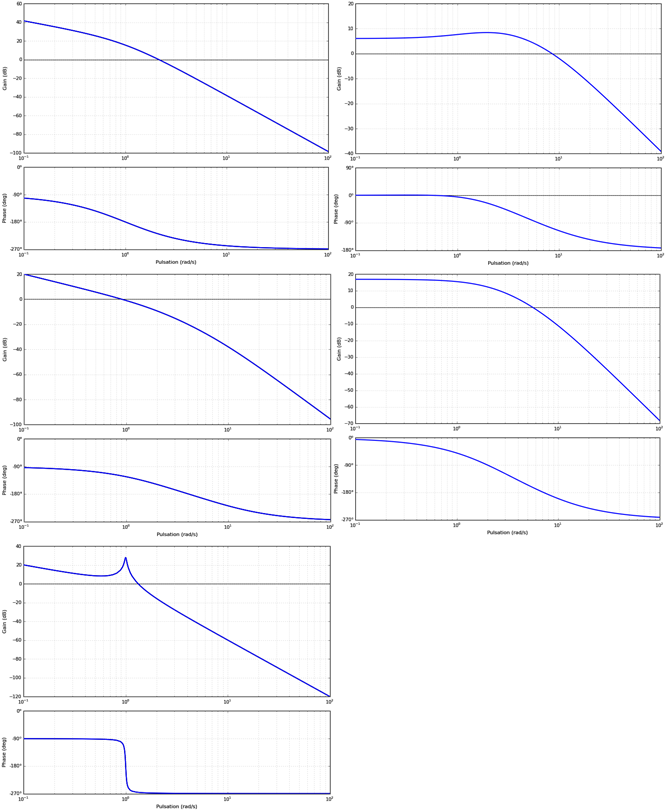
\includegraphics[width=.9\linewidth]{fig_01}
\end{center}

\subparagraph{}
\textit{Déterminer la fonction de transfert du système.}


\vspace{.5cm}

Soit la réponse à un échelon (amplitude 2,5).
\begin{center}
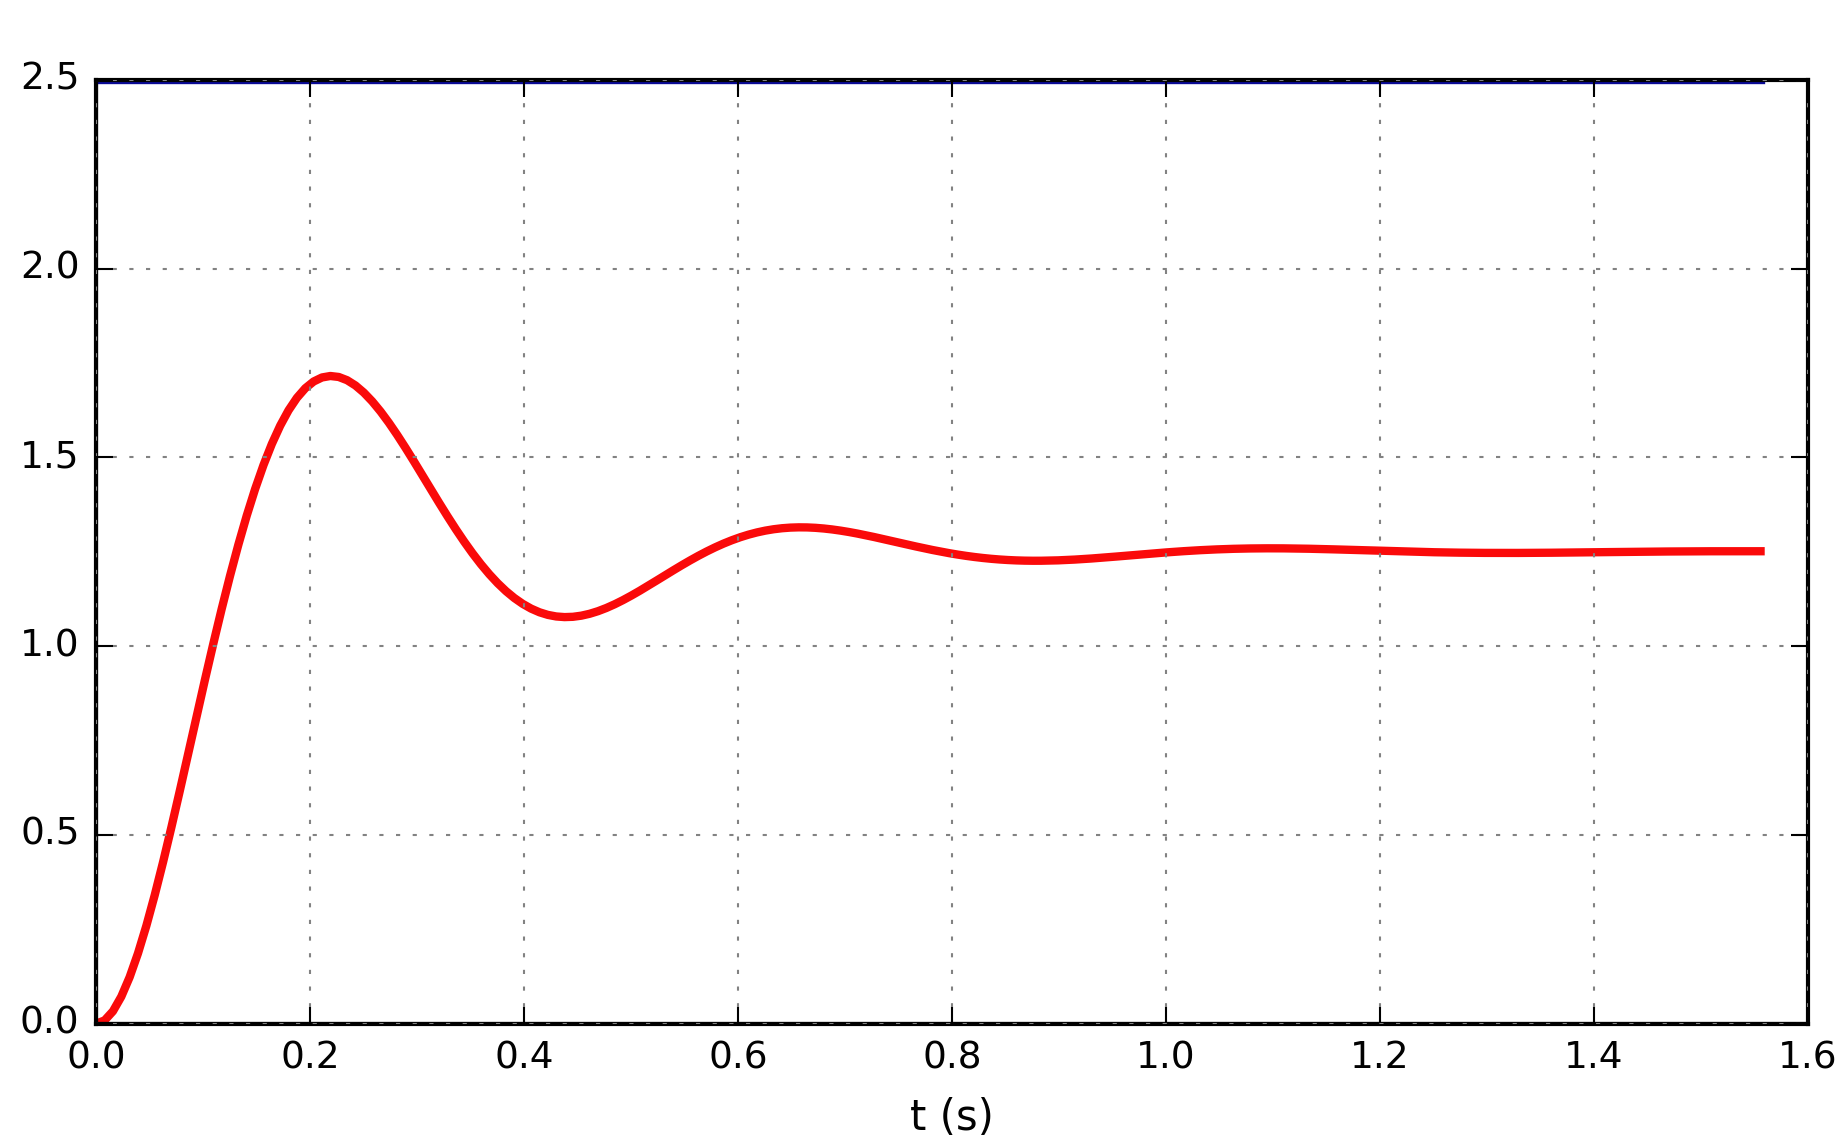
\includegraphics[width=.9\linewidth]{fig_02}
\end{center}

\subparagraph{}
\textit{Déterminer la fonction de transfert du système.}

